\documentclass[11pt]{article}
\pdfinfoomitdate=1
\pdftrailerid{}
\pdfsuppressptexinfo=15
\usepackage[T1]{fontenc}
\usepackage{lmodern}
\usepackage[a4paper,margin=29mm]{geometry}
\usepackage{amsmath,amssymb,amsthm,mathtools}
\usepackage{needspace,etoolbox}
\usepackage{microtype}
\usepackage{tikz}
\usetikzlibrary{arrows.meta,positioning,calc,decorations.pathreplacing}
\usepackage[numbers,sort&compress]{natbib}
\usepackage{xurl}
\usepackage[colorlinks=true,linkcolor=blue!45!black,citecolor=blue!45!black,urlcolor=blue!45!black]{hyperref}
\usepackage[nameinlink,noabbrev,capitalise]{cleveref}
\newtheorem{theorem}{Theorem}[section]
\newtheorem{proposition}[theorem]{Proposition}
\newtheorem{lemma}[theorem]{Lemma}
\newtheorem{corollary}[theorem]{Corollary}
\theoremstyle{definition}
\newtheorem{definition}[theorem]{Definition}
\theoremstyle{remark}
\newtheorem{remark}[theorem]{Remark}
\AtBeginEnvironment{theorem}{\Needspace{4\baselineskip}}
\AtBeginEnvironment{proposition}{\Needspace{4\baselineskip}}
\AtBeginEnvironment{lemma}{\Needspace{4\baselineskip}}
\newcommand{\C}{\mathbb C}
\newcommand{\F}{\mathbb F}
\newcommand{\Z}{\mathbb Z}
\newcommand{\PP}{\mathbb P}
\DeclareMathOperator{\im}{im}
\DeclareMathOperator{\Aut}{Aut}
\DeclareMathOperator{\End}{End}
\DeclareMathOperator{\id}{id}
\DeclareMathOperator{\cl}{cl}
\setlength{\emergencystretch}{2em}
\hyphenation{OpenAI}
\setcounter{tocdepth}{2}
\hypersetup{pdftitle={A surface counterexample to Shafarevich holomorphic convexity},pdfauthor={OpenAI}}
\title{A surface counterexample to Shafarevich holomorphic convexity}
\author{OpenAI}
\date{September 23, 2026}
\begin{document}
\maketitle
\begin{abstract}
We construct a smooth connected projective complex surface whose universal
cover is not holomorphically convex. This disproves the Shafarevich
conjecture on holomorphic convexity in complex dimension two.
\end{abstract}
\tableofcontents
\clearpage
\section{Introduction}
\label{sec:introduction}

Shafarevich asked whether the universal cover of a complete algebraic
variety is holomorphically convex \citep{Shafarevich1974}.
We follow the formulation reproduced by
\citet[pp.~135--137]{LasellRamachandran1996}, who locate the question
on p.~407 of Shafarevich's book.
We use its usual smooth-projective formulation, called the
\emph{Shafarevich conjecture on holomorphic convexity}: the universal
cover of every smooth connected projective complex variety is
holomorphically convex. For a complex manifold $V$ and a nonempty compact set $K\subset V$, its \emph{holomorphic hull} is
\[
 \widehat K_V=\{v\in V: |g(v)|\leq\sup_K|g|
                    \text{ for every }g\in\mathcal O(V)\}.
\]
Holomorphic convexity means that every such hull is compact. We disprove the conjecture in complex dimension two.

\begin{theorem}\label{thm:main}
There is a smooth connected projective complex surface $X$ containing a connected nodal curve $Z_0$ with smooth rational irreducible components such that
\[
 \im\bigl(\pi_1(Z_0)\longrightarrow\pi_1(X)\bigr)
 \quad\text{is infinite}.
\]
In the simply connected universal cover of $X$, a connected component above $Z_0$ is a closed, connected, noncompact, locally finite union of compact rational curves. The holomorphic hull of any one of its points is noncompact. In particular, this universal cover is not holomorphically convex.
\end{theorem}

\subsection{Earlier approaches and the obstruction}

The conjecture connects projective geometry with the analytic geometry
of covering spaces. Gurjar and Shastri proved it for smooth projective
elliptic surfaces \citep[Theorem~2(ii)]{GurjarShastri1985}, and
Katzarkov proved it for smooth projective varieties with virtually
nilpotent fundamental group \citep{Katzarkov1997}.
Eyssidieux proved holomorphic convexity for the cover defined by the
intersection of the kernels of all reductive complex representations
of a fixed rank \citep{Eyssidieux2004}. Eyssidieux, Katzarkov, Pantev
and Ramachandran then established the universal-cover conclusion for
smooth projective varieties whose fundamental groups admit faithful
finite-dimensional complex representations
\citep{EyssidieuxKatzarkovPantevRamachandran2012}.
Campana, Claudon and Eyssidieux extended this linear Shafarevich
theorem to compact K\"ahler manifolds
\citep{CampanaClaudonEyssidieux2015}.

Recent results extend this theory beyond smooth projective varieties.
Deng and Yamanoi, with an appendix joint with Katzarkov, proved the
fixed-rank reductive-cover conclusion for normal projective varieties
\citep[Theorem~C(i)]{DengYamanoi2024}. Bakker, Brunebarbe and Tsimerman
proved that, for a connected normal algebraic space whose fundamental
group has a finite-dimensional complex representation with finite
kernel, the universal cover is a dense analytic-Zariski open subset
of a holomorphically convex complex space
\citep[Theorem~1.1]{BakkerBrunebarbeTsimerman2026}. This last conclusion
concerns a partial compactification of the universal cover.

The geometric reduction approach seeks to contract subvarieties for which
the fundamental group of the normalization has finite image in the ambient
fundamental group. Koll\'ar's rational Shafarevich maps
and Campana's meromorphic $\Gamma$-reduction address this problem through
sufficiently general points \citep[\S1]{Kollar1993}
\citep[Theorem~3.5 and Definition~3.8]{Campana1994}.
Such generic reductions do not by themselves provide a proper holomorphic
map from the entire universal cover to a Stein space.

The obstruction used in the present construction is classical.
Lasell and Ramachandran \citep[pp.~136--137]{LasellRamachandran1996}
and Katzarkov and Ramachandran
\citep[pp.~527--528]{KatzarkovRamachandran1998} explain why a
connected curve can obstruct holomorphic convexity when its normalized
components have finite fundamental-group image but the curve itself has
infinite image. A connected lift then has compact irreducible
components but is itself noncompact. Such a curve is called an
\emph{infinite Nori string}
\citep[arXiv version, Definition~3]{ColtoiuJoita2011}.
Every holomorphic function is constant on each compact component,
and connectedness makes these constants agree. A closed infinite Nori
string therefore cannot lie in a holomorphically convex space.
For our rational components the individual fundamental groups are
trivial; the decisive issue is the image of the loops in the incidence
graph of their whole nodal union.

Bogomolov and Katzarkov proposed constructions from degenerating
curves and quotients of their fundamental groups in which this
obstruction would occur if the resulting geometric quotient remained
infinite after all required relations
\citep[author manuscript, \S4.1, Lemma~4.2 and Conjecture~4.1]{BogomolovKatzarkov1998}.
That infinitude assertion remained conditional. Eyssidieux and Funar
subsequently proved holomorphic convexity for the associated
uniform-ramification construction from semistable families of curves
of genus at least two, outside explicit finite exceptional ranges
\citep[Theorems~1.2 and~6.18]{EyssidieuxFunar}.

The construction here follows the same broad passage from a family
of curves to a group quotient and then to a projective surface.
Its input is a marked genus-zero family, with both horizontal marked
sections and vertical boundary components. A \emph{meridian} is the
boundary of a small disk transverse to a divisor. We kill the meridians of
one distinguished fiber and impose high powers of the remaining
boundary meridians only after compactification. The argument must
establish both infinitude of this particular quotient and its
survival in the final surface. The weighted presentation proves the
first assertion; finite detection of entire local boundary-group
images, followed by transfer to the compact rational fiber, proves
the second. These are the steps developed below.

\subsection{Consequences and comparisons}

By the linear Shafarevich theorem, the fundamental group of the surface
in \Cref{thm:main} has no faithful finite-dimensional complex
representation. Two further comparisons concern restrictions on the
surface and on its universal cover.

A smooth compact K\"ahler manifold $M$ is \emph{special} in Campana's
sense if no holomorphic line bundle $L$ admits a nonzero map
$L\to\Omega_M^p$ with $\kappa(M,L)=p$ for any $1\le p\le\dim M$;
here $\kappa$ denotes Iitaka dimension
\citep[Theorem~2.27]{Campana2004}. The abelianity theorem for
special compact K\"ahler manifolds gives a virtually abelian
fundamental group, and hence a faithful finite-dimensional complex
representation. The compact K\"ahler linear theorem therefore makes
their ordinary universal covers holomorphically convex
\citep[Corollary~1.4]{OpenAIAbelianity2026}.
Consequently the surface in \Cref{thm:main} is not special.

A subset of a complex projective variety is \emph{semialgebraic}
if it is given in affine charts by finite Boolean combinations of
real polynomial equalities and inequalities. The ordinary universal
cover of our surface is not biholomorphic to a semialgebraic open
subset of a projective variety, with openness in the complex
topology: such a presentation would imply holomorphic convexity by
\citep[Corollary~8.1]{OpenAISemialgebraicCovers2026}, contrary to
\Cref{thm:main}.

\subsection{The construction in outline}

We begin with a family of spheres with $48$ moving punctures. The family comes from multiplication by $4$ on the elliptic curve with an automorphism of order three. Near one parameter value, the punctures collide in $24$ pairs. A double base change and one blowup at each collision produce an unmarked main sphere with $24$ attached spheres, each carrying two marked points. Finite covers of these components, branched only at those points, are again rational.

The main task is to retain an infinite fundamental-group image after filling in this fiber and all other missing fibers. Three features make this possible.

First, we study the moving points on the elliptic curve before taking its sign quotient. Three explicit double covers show that monodromy changes each generator only in higher degree. Deep elements of the free parameter group therefore impose relations of arbitrarily high degree. A surjective map of the actual based fiber groups transfers these equalities to the sphere family.

Second, the multiplication cover has deck group $(\Z/4)^2$. Successive differences under its two translations give a free basis with useful degrees. A calculation with the linear terms of the sign involution selects $24$ relations that impose all sign identifications on this $48$-generator group. These relations leave a strict margin in a weighted Golod--Shafarevich inequality. That margin accommodates the deep monodromy relations and large powers of the remaining boundary loops. The weighted infinitude method builds on \citet{GolodShafarevich1964}, \citet{Golod1964}, \citet{Vinberg1965}, \citet{Ershov2011}, and \citet{ErshovJaikinZapirain2013}. The group construction takes place in inverse limits of finite 2-groups, described in \Cref{sec:weighted}.

Third, we choose the finite parameter cover and compactify the marked family. Only then do we impose high powers of the remaining boundary meridians so that their images are finite. We then choose a finite quotient that is injective on each entire local boundary-group image. In the associated cover, this lets the infinite quotient survive normalization and resolution, including every exceptional divisor. The resulting smooth projective surface retains a rational special fiber. A neighborhood deformation retraction and properness transfer the infinite image of a nearby fiber to a connected component of that rational fiber.

The two reusable mechanisms are the economical involution presentation in \Cref{prop:involution} and the finite-local-group argument in \Cref{lem:local-detection}. The former retains enough generators relative to relations for the weighted infinitude criterion; the latter extends a homomorphism from the fundamental group of a divisor complement across a smooth projective compactification of a finite cover.

We give the weighted algebra in \Cref{sec:weighted}, construct and compare the actual fiber groups in \Cref{sec:family}, and analyze the involution in \Cref{sec:involution}. \Cref{sec:quotient} constructs the infinite quotient and the compactified marked family. \Cref{sec:surface} completes the surface and its rational curve.

\subsection{Why the rational curve is enough}

The following elementary form of the compact-curve obstruction makes the last step explicit. It is the rational-curve case of the mechanism described in \citet[pp.~136--137]{LasellRamachandran1996}, \citet[pp.~527--528]{KatzarkovRamachandran1998}, and \citet[author manuscript, \S4.1]{BogomolovKatzarkov1998}.

\begin{lemma}\label{lem:rational-hull}
Let $X$ be a connected complex manifold and let $Z\subset X$ be a compact connected nodal curve whose irreducible components are smooth rational curves. If the image of $\pi_1(Z)\to\pi_1(X)$ is infinite, then every connected component $W$ of the inverse image of $Z$ in the simply connected universal cover $\widetilde X$ is closed and noncompact. It is a locally finite union of compact rational curves, and every holomorphic function on $\widetilde X$ is constant on $W$.
Consequently $\widehat{\{w\}}_{\widetilde X}$ is noncompact for every $w\in W$.
\end{lemma}

\begin{proof}
The restricted map $W\to Z$ is the connected covering corresponding to
\[
 \ker\bigl(\pi_1(Z)\longrightarrow\pi_1(X)\bigr).
\]
Thus it has infinitely many sheets. A fiber is a closed discrete infinite subset, so $W$ cannot be compact. It is closed in $\widetilde X$, since it is a connected component of the closed inverse image of $Z$.

Each rational component of $Z$ is simply connected. Its inverse image therefore consists of compact rational curves mapping isomorphically onto it. Choose an evenly covered neighborhood in $X$ of each point of $Z$, small enough that it meets $Z$ in one smooth branch or in the two branches of a node. Each lifted neighborhood meets at most one or two lifted components. These neighborhoods show that the collection is locally finite in the ambient manifold $\widetilde X$; points outside the closed inverse image have a neighborhood meeting none of it. The connected space $W$ is locally path connected; a path in it has compact image and meets only finitely many of these curves. The maximum principle makes a holomorphic function constant on each compact curve, and the constants agree at their intersections. They therefore agree throughout $W$.

For $w\in W$, this proves $W\subset\widehat{\{w\}}_{\widetilde X}$. A compact hull cannot contain the closed noncompact set $W$.
\end{proof}

\section{Weighted free pro-2 groups}
\label{sec:weighted}

We will construct an infinite quotient by comparing the weighted number of generators with the weighted number of relations. This section records the precise version of the Golod--Shafarevich argument that we use, including convergence for infinitely many relators.

\subsection{Magnus degrees and automorphisms}

A pro-2 group is an inverse limit of finite groups of order a power of two. The free pro-2 group on a finite set is the pro-2 completion of the discrete free group on that set. Let $F_d$ be free pro-2 on $g_1,\ldots,g_d$, and assign positive integer weights $w_1,\ldots,w_d$. Its Magnus expansion sends
\[
 g_i\longmapsto1+U_i
 \quad\text{in}\quad
 A=\F_2\langle\!\langle U_1,\ldots,U_d\rangle\!\rangle,
 \qquad \deg U_i=w_i.
\]
Here $A$ is the algebra of formal noncommutative power series, with the filtration $A_{\ge n}$ by weighted degree at least $n$. For $g\ne1$, let $\nu(g)$ be the least degree in $g-1$, and put $\nu(1)=\infty$.

For clarity, this expansion is faithful and gives the pro-2 topology. Each truncated algebra is finite, and its group $1+A_{>0}/A_{\ge n}$ is a finite 2-group. Conversely the augmentation ideal of $\F_2[P]$ is nilpotent for every finite 2-group $P$. To see this, induct on $|P|$, choosing a central involution $z$ when $P\ne1$. The kernel of $\F_2[P]\to\F_2[P/\langle z\rangle]$ is generated by $z-1$ and has square zero. Nilpotence follows by induction. Thus every finite 2-quotient of the free group factors through some Magnus truncation. This proves faithfulness on the pro-2 completion and cofinality of the truncations. Positive finite weights give the same topology as ordinary degree.

Multiplication of series gives
\begin{equation}\label{eq:degree-rules}
 \nu(gh)\ge\min\{\nu(g),\nu(h)\},\qquad
 \nu([g,h])\ge\nu(g)+\nu(h),\qquad
 \nu(g^{2^e})\ge2^e\nu(g).
\end{equation}
We use either commutator convention, since only its degree matters. The last inequality follows from $g^{2^e}-1=(g-1)^{2^e}$ in characteristic two.

\begin{lemma}[Substitution]\label{lem:substitution}
Suppose an automorphism $\alpha$ of $F_d$ satisfies
\[
 \nu\bigl(\alpha(g_i)g_i^{-1}\bigr)\ge w_i+a
 \quad(1\le i\le d)
\]
for an integer $a\ge1$. Then its continuous action on $A$ satisfies
\[
 (\alpha-\id)(A_{\ge n})\subset A_{\ge n+a}.
\]
More generally, substitution of degree-raising operators for Magnus variables is well defined whenever the operator assigned to a variable of weight $w$ raises degree by at least $w$.
\end{lemma}

\begin{proof}
The hypothesis says that $\alpha(U_i)-U_i$ has degree at least $w_i+a$. Expand the difference between a monomial and its substituted image. Every summand replaces at least one factor by an error of at least $a$ additional degrees. The estimate follows for polynomials and then for series by completeness. For operator substitution, a word of weighted degree $n$ raises degree by at least $n$; hence only finitely many words contribute in each finite truncation. Multiplication and composition respect these substitutions.
\end{proof}

We also use the following basis criterion. The \emph{Frattini quotient} of a finitely generated pro-2 group $G$ is
\[
 G/\overline{G^2[G,G]},
\]
an $\F_2$-vector space. Elements whose images span this space topologically generate $G$: otherwise their closed generated subgroup has proper image in a finite 2-quotient, and is contained in a maximal subgroup of index two there, contradicting the span. Consequently, $d$ elements of $F_d$ whose Frattini images form a basis are again a free pro-2 basis. Indeed, they define a surjective endomorphism of $F_d$, and every finitely generated profinite group is Hopfian. For the latter assertion, a surjective endomorphism permutes, by inverse image, the finite set of open normal subgroups of any fixed index. Its kernel therefore lies in every open normal subgroup and is trivial.

\subsection{The infinitude inequality}

The infinitude method originates in the work of \citet{GolodShafarevich1964}; \citet{Vinberg1965} developed its filtered form. For the weighted completed-algebra inequality and its pro-$p$ consequence, see \citet[Theorem~2.1 and Corollary~2.2]{Ershov2011}. The more general language of positive weighted deficiency is developed by \citet[arXiv version, Corollary~4.4]{ErshovJaikinZapirain2013}. We include the filtered proof needed here to specify exactly the completion and the infinite-relator convention.

\begin{lemma}[Weighted infinitude criterion]\label{lem:weighted-gs}
Let $F_d$ have the weighted basis above, and let $(r_\lambda)$ be a finite or countable family of relators with positive integer bounds $v_\lambda$ satisfying
\[
 \nu(r_\lambda)\ge v_\lambda\ge1.
\]
Assume only finitely many $v_\lambda$ lie below any fixed bound. If, for some $0<t<1$, the relator series converges and
\begin{equation}\label{eq:gs-criterion}
 1-\sum_{i=1}^d t^{w_i}+\sum_\lambda t^{v_\lambda}<0,
\end{equation}
then the quotient of $F_d$ by the closed normal subgroup generated by all $r_\lambda$ is infinite.
\end{lemma}

\begin{proof}
Let $I\subset A$ be the closed two-sided ideal generated by $f_\lambda=r_\lambda-1$, and let $R=A/I$ with its quotient filtration. Put
\[
 C(n)=\dim_{\F_2}R/R_{\ge n}\quad(n\ge1),
 \qquad C(n)=0\quad(n\le0).
\]
First-letter decomposition gives a surjective map
\[
 \bigoplus_i R/R_{\ge n-w_i}\longrightarrow
 R_{>0}/R_{\ge n},\qquad
 (b_i)_i\longmapsto\sum_i U_i b_i.
\]
Its kernel has dimension at most $\sum_\lambda C(n-v_\lambda)$. Here is the filtered justification. Write $f_\lambda=\sum_i U_i f_{i\lambda}$. A vector in the kernel can be lifted to series whose first-letter sum lies in $I+A_{\ge n}$. Subtracting the first-letter decomposition of the degree-at-least-$n$ term does not change the truncated vector, so the sum may be taken in $I$. For a product $a f_\lambda h$, the positive-degree part of $a$ contributes first-letter coefficients that vanish in $R$; its constant part contributes
\[
 (\overline{f_{i\lambda}})_i\,\bar h.
\]
This vector has shifted degree at least $v_\lambda$. Only $\bar h$ modulo $R_{\ge n-v_\lambda}$ matters. These vectors therefore span a space of dimension at most $\sum_\lambda C(n-v_\lambda)$. Closure adds nothing to a span in a finite-dimensional truncation. Since $\dim R_{>0}/R_{\ge n}=C(n)-1$, we obtain
\begin{equation}\label{eq:cumulative-gs}
 C(n)-\sum_i C(n-w_i)+\sum_\lambda C(n-v_\lambda)\ge1.
\end{equation}

Suppose the stated pro-2 quotient were finite, of order $m$. Its image spans every truncated algebra $R/R_{\ge n}$: the variables are the images of $g_i-1$, and their products are linear combinations of group elements. The group map to each truncated unit group kills the relators, hence factors through that quotient. Thus $C(n)\le m$ for all $n$.
Multiply \eqref{eq:cumulative-gs} by $t^{n-1}$ and sum over $n\ge1$. Boundedness of $C(n)$ and convergence of the relator series justify the sums. This gives
\[
 \left(1-\sum_i t^{w_i}+\sum_\lambda t^{v_\lambda}\right)
 \sum_{n\ge1}C(n)t^{n-1}\ge\frac1{1-t},
\]
contradicting \eqref{eq:gs-criterion}.
\end{proof}

The use of lower bounds $v_\lambda$ makes the criterion convenient: increasing an actual relator degree can only improve the inequality. In the construction below, the inexpensive relations impose a geometric involution. The remaining relations will be pushed arbitrarily far into the filtration.

\section{A family of paired punctures}
\label{sec:family}

We construct a family of spheres with 48 marked points.  Near one missing
parameter value these points form 24 disjoint pairs.  The purpose of this
section is to relate the actual based monodromy of the family to an action
on a free group whose weighted Magnus degree it raises.  We also identify
the quotient obtained by killing the loops around the pairs.

\subsection{The family and its torus cover}

Put
\[
 E=\C/(\Z+\Z\omega),\qquad \omega^3=1,\quad \omega\ne1,
 \qquad \iota(z)=-z.
\]
Let $q:E\to E/\langle\iota\rangle=\PP^1$ be the quotient map.
Multiplication by $\omega$ and by $4$ induce maps $\bar\omega$ and $f$
on $\PP^1$, respectively.  Thus
\[
 q\circ[4]=f\circ q,\qquad q\circ[\omega]=\bar\omega\circ q.
\]
Our parameter curve is
\begin{equation}\label{eq:parameter-base}
 B=\PP^1\setminus
 \bigl(q(E[2])\cup q(\ker(1-\omega))\bigr).
\end{equation}
For $s\in B$, let $\mathcal A_s$ be the following subset of the fiber
sphere:
\begin{equation}\label{eq:sphere-markings}
 \mathcal A_s=\{z\in\PP^1:f(z)=\bar\omega^j s
                  \text{ for some }j\in\{0,1,2\}\}.
\end{equation}

\begin{lemma}\label{lem:family}
The complement defining $B$ consists of five points.  The sets
$\mathcal A_s$ form 48 disjoint points varying as an \emph{\'{e}tale
multisection}: locally on $B$ they are the graphs of 48 distinct
holomorphic functions.  The point $q(0)$ belongs to no $\mathcal A_s$.
If $e_0\in E[2]\setminus\{0\}$ and $s_*=q(e_0)$, then as $s\to s_*$
the markings collide in 24 pairs, each at a simple ramification point
of $f$.
\end{lemma}

\begin{proof}
The group $\ker(1-\omega)$ has order three.  Its two nonzero points are
exchanged by $\iota$, and its intersection with $E[2]$ is $\{0\}$.
This gives the five excluded values.  A fixed point of $\bar\omega$
lifts to a point satisfying $\omega z=\pm z$; since $1+\omega$ is a
unit in $\Z[\omega]$, all such values are excluded by
\eqref{eq:parameter-base}.  The three targets in
\eqref{eq:sphere-markings} are therefore distinct.  They avoid
$q(E[2])$, which contains the critical values of the degree-16 map $f$.
Also $f(q(0))=q(0)$, so $q(0)$ gives a section of the complement.

The three points $e_j=\omega^j e_0$ are the distinct nonzero elements
of $E[2]$.  A point $p\in E$ with $[4]p=e_j$ is not two-torsion.
Consequently $q$ is unramified at $p$, $[4]$ is \'etale there, and $q$
is simply ramified at $e_j$.  Thus $f$ has simple ramification at
$q(p)$.  The sixteen points above each $e_j$ are paired freely by
$\iota$, giving eight collisions for each $j$ and 24 in total.
\end{proof}

Choose henceforth $e_0\in E[2]\setminus\{0\}$ and put $s_*=q(e_0)$.
Fix $s_0\in B$ sufficiently close to $s_*$, and choose
$x_0\in q^{-1}(s_0)$ close to $e_0$.  The six points
$\pm\omega^j x_0$ lie, two at a time, in disjoint $\iota$-invariant
disks $D_j$ about $e_j$, none containing zero.  Write
\[
 T=E\setminus\{\pm\omega^j x_0:0\le j\le2\},\qquad
 F=\pi_1(T,0),\qquad \Gamma=\pi_1(B,s_0).
\]
The group $\Gamma$ is free of rank four.  In the core
$E\setminus\bigcup_j\operatorname{int}D_j$, choose handle generators
$x,y$ representing the lattice basis $1,\omega$.  Choose based
meridians $a_j,a_j^-$ about the two punctures in
$D_j$, with core access paths, so that its boundary loop is
$c_j=a_ja_j^-$.  The choices and ordering can be made so that the
surface relation is $[x,y]c_0c_1c_2=1$.  Hence $F$ is free on
\begin{equation}\label{eq:torus-free-basis}
 x,y,a_0,a_1,a_2,c_0,c_1.
\end{equation}
Give the first five generators weight one and the last two weight
two.  Let $\nu_F$ be the resulting Magnus valuation on the pro-2
completion $\widehat F$.  The surface relation gives $\nu_F(c_2)\ge2$.

The multiplication map $[4]$ restricts to an unramified cover of $T$.
Its deck group and based covering subgroup are
\[
 H=(\Z/4)^2,\qquad
 K=\ker\bigl(F\longrightarrow H\bigr),
\]
where the map records the two handle coordinates modulo four.
Thus $K$ is free of rank $1+16(7-1)=97$.  Its source is
\[
 T^{(4)}=[4]^{-1}(T),\qquad K=\pi_1(T^{(4)},0),
\]
the torus with the 96 preimages of the six punctures removed.
Quotienting $T^{(4)}$ by $\iota$ gives
\[
 S=\PP^1\setminus\mathcal A_{s_0},\qquad
 \Pi=\pi_1(S,q(0)).
\]
We identify $K$ with the based fundamental group of the source torus
through $[4]$ and denote by $p:K\to\Pi$ the map induced by $q$.
The group $\Pi$ is free of rank 47.

The two fiber groups serve different purposes. The torus group $F$ has a
small basis on which monodromy can be controlled; the sphere group $\Pi$
is the fundamental group of the geometric fiber used in the surface.
The covering subgroup $K$ will connect these two descriptions. Keeping
this connection based, rather than only up to an inner automorphism,
is essential when we impose monodromy relations.

\subsection{Actual based monodromy}

Following $x_0$ over a loop $m\in\Gamma$ ends at
$(-1)^{\epsilon(m)}x_0$; this defines a character
$\epsilon:\Gamma\to\Z/2$.  Follow also the six points
$\pm\omega^j x_0$.  Their motion extends to an isotopy $H_u$ of the
torus which fixes zero and commutes with $\iota$.  Indeed, subdivide
the path into motions in disjoint small disks, prescribe a vector
field in one disk of each sign pair, extend it equivariantly to the
other, and use bump functions supported away from zero. Every $H_u$
fixes all four points of $E[2]$ pointwise: commutation with $\iota$
preserves this discrete fixed-point set, and an isotopy starting at the
identity cannot permute it. Define the
corrected endpoint and its based action by
\begin{equation}\label{eq:corrected-monodromy}
 \iota^{\epsilon(m)}H_1,
 \qquad \varphi_m\in\Aut(F).
\end{equation}
The correction fixes each of the six punctures individually; this
is what \emph{pure} means here.

\begin{proposition}\label{prop:based-monodromy}
The actions $\varphi_m$ form a homomorphism
$\Gamma\to\Aut(F)$, are pure, and commute with $\iota_*$.
They preserve $K$.  If $\beta_m\in\Aut(\Pi)$ is the actual based
monodromy of the punctured sphere family, then
\begin{equation}\label{eq:actual-monodromy-square}
 p\circ\varphi_m|_K=\beta_m\circ p.
\end{equation}
Moreover, $p:K\to\Pi$ is surjective.
\end{proposition}

\begin{proof}
Two extensions of the same point motion differ by an isotopy fixing
the initial punctures and zero.  Their endpoint actions therefore
agree.  The disk construction also extends homotopies of parameter
paths.  With loop composition chosen to agree with composition of
the endpoint actions, uncorrected monodromy is a homomorphism.
All its maps commute with $\iota$, and $\epsilon$ is a character,
so the corrected actions also compose.

The uncorrected endpoint acts trivially on the homology of the
closed torus; the correction acts there by a sign.  It therefore
preserves the handle-coordinate kernel $K$ and lifts uniquely
through $[4]$ fixing zero.  The lift commutes with $\iota$ by
uniqueness: both compositions lift the same map and fix zero.
Requiring this fixed basepoint also excludes any nontrivial deck
translation. Write $\widetilde H_u$ for the lift of $H_u$ through
$[4]$ starting at the identity; it fixes zero and gives the actual
motion of the $96$ punctures upstairs. The zero-fixed lift of the
corrected endpoint is $\iota^{\epsilon(m)}\widetilde H_1$, because
$[4]$ commutes with sign. After quotienting by sign, this endpoint
is the endpoint induced by $\widetilde H_u$, hence gives the actual
based sphere monodromy. This proves \eqref{eq:actual-monodromy-square}.

For surjectivity, represent a loop in $S$ based at $q(0)$ by a path
which avoids the four branch values of $q$ except at its endpoints.
Its open interval lifts through the ordinary two-sheeted cover
away from those values.  Both lifted endpoints tend to zero,
the unique point above $q(0)$.  Thus the lift is a based loop in
the source punctured torus, as required.
\end{proof}

\subsection{Three invariant double covers}

We next prove that $\varphi_m-\id$ raises the weighted degree on
$\widehat F$.  The only delicate first step is its action in degree
one.  Three double covers of the moving torus complement make this
action explicit.

\begin{lemma}\label{lem:degree-one}
Every $\varphi_m$, and also $\iota_*$, acts as the identity on
the weighted degree-one quotient
$V=\widehat F/\{g:\nu_F(g)\ge2\}$.
\end{lemma}

\begin{proof}
The vector space $V$ over $\F_2$ has the five basis classes
$x,y,a_0,a_1,a_2$.  Two characters of $F$ are obtained from the
handle coordinates modulo two.  Uncorrected monodromy preserves
them, and $\iota$ preserves them modulo two.

Choose an affine coordinate on the quotient sphere with
$q(0)=\infty$, using the same letter $q$ for its pullback to $E$.
It is an even meromorphic function with a double pole at zero.
Normalize its leading coefficient to one in an additive local
coordinate $v$ at zero, so that
$v(\iota z)=-v(z)$ and $q(z)=v(z)^{-2}+O(1)$.
For $j=0,1,2$, consider over the moving torus complement the cover
\begin{equation}\label{eq:character-cover}
 Y_j^2=q(z)-\bar\omega^j s.
\end{equation}
Here $s$ and $\bar\omega^j s$ are expressed in the chosen affine
coordinate.  The right side has simple zeros precisely at the
two removed $j$-punctures.  The cover is unramified elsewhere,
including at zero: with $\eta=vY_j$, its local equation is
\[
 \eta^2=v^2(q(z)-\bar\omega^j s)=1+O(v^2).
\]
Thus the points $\eta=1$ and $\eta=-1$ over zero give two global
lifts of the fixed basepoint section throughout $B$.

Let $\chi_j:F\to\F_2$ be the character of this double cover on the
fiber over $s_0$.  A cover of the entire family with a lifted
basepoint section gives an extension of $\chi_j$ to the fundamental
group of its total space.  Conjugating a fiber loop by the section
loop does not change its value in $\F_2$.  Hence uncorrected based
monodromy preserves $\chi_j$.  Sign has the lift
\[
 (z,Y_j)\longmapsto(-z,-Y_j).
\]
This lift fixes each selected sheet over zero, because both $v$
and $Y_j$ change sign and $\eta=vY_j$ does not.  It follows that
$\iota_*$ also preserves $\chi_j$, and therefore so does the
corrected action $\varphi_m$.

The character $\chi_j$ takes value one on $a_j$ and $a_j^-$ and
zero on the other puncture meridians.  In particular it vanishes
on all $c_i$ and factors through $V$.  The three characters
$\chi_j$, together with the two handle characters, form a basis
of $V^*$: evaluation on the five displayed generators has an
invertible block triangular matrix.  Their common kernel is therefore
$\{g:\nu_F(g)\ge2\}$.  Since all five characters are preserved,
this kernel is preserved and the two induced actions on $V$ are trivial.
\end{proof}

\begin{proposition}\label{prop:monodromy-raising}
For every $m\in\Gamma$, the induced operator
$\varphi_m-\id$ on the weighted completed Magnus algebra of
$\widehat F$ raises degree by at least one.
\end{proposition}

\begin{proof}
By \Cref{lem:degree-one}, the changes of the five weight-one
generators in \eqref{eq:torus-free-basis} have valuation at least
two.  It remains to check the two weight-two boundaries.
Fix one pair, writing $a=a_j$ and $a^-=a_j^-$.
Pureness gives $\varphi_m(a)=waw^{-1}$ for some $w\in F$.
Choose $d\in F$ with $\iota_*(a)=d a^-d^{-1}$.
Commutation with $\iota_*$ yields
\[
 \varphi_m(a^-)=w'a^-(w')^{-1},\qquad
 w'=\varphi_m(d)^{-1}\iota_*(w)d.
\]
By \Cref{lem:degree-one}, $w'w^{-1}$ has valuation at least two.
Replacing $w'$ by $w$ in the conjugation of $a^-$ therefore changes
it by an element of valuation at least three.  On the other hand,
conjugating $c_j=aa^-$ by $w$ changes it by valuation at least
$1+\nu_F(c_j)\ge3$.  It follows that
\[
 \nu_F\bigl(\varphi_m(c_j)c_j^{-1}\bigr)\ge3.
\]
The degree-raising substitution rule of \Cref{lem:substitution}
now applies to the entire weighted free basis.
\end{proof}

\subsection{Pinching the pairs and passing to the sphere}

We have obtained a degree-raising action on the seven-generator
torus group. We now collapse the lifted core to obtain a free group
on the individual puncture pairs. This construction will identify
both the quotient map from $K$ and its compatibility with the
\emph{actual} sphere group $\Pi$.

Write
\[
 T_{\mathrm{core}}=E\setminus\bigcup_j\operatorname{int}D_j,
 \qquad T_{\mathrm{core}}^{(4)}=[4]^{-1}(T_{\mathrm{core}}).
\]
The lifted core $T_{\mathrm{core}}^{(4)}$ is connected, because the
handle loops in $T_{\mathrm{core}}$ map onto $H$. Its complementary disks are indexed by
$(h,j)\in H\times\{0,1,2\}$. For each $j$, choose the index-zero
disk to be the one reached by lifting the chosen access path of
$a_j$ from zero; use deck translations to label the others.
All four fixed points of sign lie in $T_{\mathrm{core}}^{(4)}$, since multiplication
by four sends them to zero, outside every $D_j$.

Collapsing $T_{\mathrm{core}}^{(4)}$ kills its fundamental group, including every
disk boundary. By van Kampen, the resulting quotient of $K$ is
free on one positive meridian for each of the $48$ disks: in each
two-puncture disk, killing the boundary makes the negative meridian
the inverse of the positive one. Let $L$ be the pro-2 completion
of this free group, with generators $a_{h,j}$. Paths in the lifted
core disappear under collapse, so these generators do not depend
on the remaining choices of core access paths. Deck translations
induce the coordinate shifts $T_1,T_2$ on $L$.

We also denote the corresponding elements of the factor $H$ in
$L\rtimes H$ by $T_1,T_2$. Define
\begin{equation}\label{eq:torus-substitution}
 \begin{aligned}
 \Phi:F&\longrightarrow L\rtimes H,\\
 x&\longmapsto T_1,& y&\longmapsto T_2,&
 a_j&\longmapsto a_{0,j},& c_0,c_1&\longmapsto1.
 \end{aligned}
\end{equation}
The shifts commute and have order four, so $c_2$ also maps to one.
On the core group, $\Phi$ is exactly the $H$-valued covering
character. It therefore kills $\pi_1(T_{\mathrm{core}}^{(4)},0)\subset K$.
A positive meridian in disk $(h,j)$ can be based using the lift
of $u a_j u^{-1}$, where $u$ is a core loop with handle coordinate
$h$; its image under $\Phi$ is exactly $a_{h,j}$. Thus
$\Phi|_K:K\to L$ is the core-collapse map just constructed,
followed by pro-2 completion. Its image contains the discrete free
group on the $a_{h,j}$ and is dense in $L$.

Sign preserves the lifted core and pairs its complementary disks
freely: their centers map to nonzero two-torsion, whereas $[4]$
kills the source two-torsion. Let $b_j\in H$ be the index of the
negative of the chosen index-zero center. Sign takes a positive
puncture in disk $(h,j)$ to the negative puncture in disk
$(b_j-h,j)$. Since both core access paths and disk boundaries
have been killed, its induced action is exactly
\begin{equation}\label{eq:pinched-involution}
 \sigma(a_{h,j})=a_{b_j-h,j}^{-1}.
\end{equation}
If the index-zero center is represented by $v/4$, with
$v\bmod(\Z+\Z\omega)=e_j$, then $b_j$ is represented, up to
the deck-coordinate convention, by $-2v$ modulo
$4(\Z+\Z\omega)$. Since $e_j$ is nonzero two-torsion,
\begin{equation}\label{eq:odd-displacement}
 b_j\bmod2H\ne0.
\end{equation}

\begin{lemma}\label{lem:pinched-sphere}
Let $\Pi_{\mathrm{pair}}$ be the quotient of $\Pi$ obtained by
killing the boundary loops of its 24 two-puncture disks.
It is free of rank 24, and its pro-2 completion is naturally
\begin{equation}\label{eq:pinched-sphere-group}
 \widehat{\Pi_{\mathrm{pair}}}
 \simeq L/\overline{\langle\!\langle
              \sigma(g)g^{-1}:g\in L
                    \rangle\!\rangle}.
\end{equation}
More precisely, let $\lambda:L\twoheadrightarrow R$ be a continuous
quotient of pro-2 groups satisfying $\lambda\sigma=\lambda$.
There is a homomorphism $\theta:\Pi\to R$ with dense image and
\begin{equation}\label{eq:pinching-square}
 \theta p=\lambda\Phi|_K.
\end{equation}
For $m\in\Gamma$, the condition
\begin{equation}\label{eq:torus-equalizer-condition}
 \lambda\Phi(\varphi_m(k))=\lambda\Phi(k)
 \qquad(k\in K)
\end{equation}
implies $\theta\beta_m=\theta$ on the entire unpinched group
$\Pi$.
\end{lemma}

\begin{proof}
Each sign-paired pair of torus disks projects to one two-puncture
disk on the sphere, and either disk maps homeomorphically to it.
The image $q(T_{\mathrm{core}}^{(4)})$ is the sphere exterior, a sphere with $24$
holes. Killing its boundary loops kills its fundamental group,
so the quotient defining $\Pi_{\mathrm{pair}}$ is the quotient
induced by collapsing this exterior. Van Kampen identifies it
with the free group on one meridian per projected disk.

The map $q$ commutes with the two core collapses, with the
basepoints in their respective cores. Upstairs there is one
cyclic generator per disk, and sign identifies them in pairs by
$a_{h,j}=a_{b_j-h,j}^{-1}$. This accounts for the entire quotient:
every fixed point of sign is already in the collapsed core, and
either disk in each remaining pair maps homeomorphically to the
corresponding sphere disk. Passing to pro-2 completions proves
\eqref{eq:pinched-sphere-group}. The based collapse diagram then
gives the dense map $\theta$ and the exact identity
\eqref{eq:pinching-square}.

Finally, \Cref{prop:based-monodromy} and
\eqref{eq:torus-equalizer-condition} give
\[
 \theta\beta_m p
 =\theta p\varphi_m|_K
 =\lambda\Phi\varphi_m|_K
 =\lambda\Phi|_K
 =\theta p.
\]
The map $p$ is surjective, so $\theta\beta_m=\theta$.
This argument does not require the monodromy to preserve the
kernel of the pair-pinching map.
\end{proof}

The maps just constructed are summarized in \Cref{fig:group-maps}.
\begin{figure}[htbp]
\centering
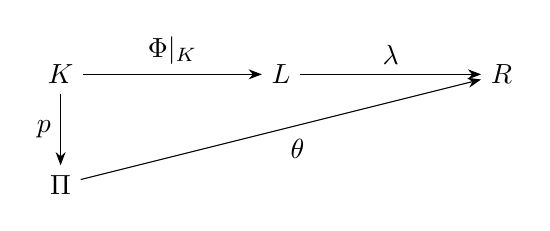
\begin{tikzpicture}[baseline=(current bounding box.center),>=Stealth]
 \node (K) at (0,1) {$K$};
 \node (L) at (2.8,1) {$L$};
 \node (R) at (5.6,1) {$R$};
 \node (Pi) at (0,-0.4) {$\Pi$};
 \draw[->] (K) -- node[above] {$\Phi|_K$} (L);
 \draw[->] (L) -- node[above] {$\lambda$} (R);
 \draw[->] (K) -- node[left] {$p$} (Pi);
 \draw[->] (Pi) -- node[below right] {$\theta$} (R);
\end{tikzpicture}
\caption{The actual sphere group $\Pi$ maps to every pro-$2$ quotient
$R$ of $L$ on which sign acts trivially. The triangle records
$\theta p=\lambda\Phi|_K$. The map $p$ is surjective and $\Phi|_K$
has dense image. Monodromy is compared on $K$ and $\Pi$ before it is
passed to $R$.}
\label{fig:group-maps}
\end{figure}


We conclude with two properties of the finite geometric monodromy
which will control a parameter cover.  Let $\gamma_*\in\Gamma$ be
the positively oriented local circuit around $s_*$ based at the
nearby point $s_0$.

\begin{lemma}\label{lem:finite-geometric-monodromy}
The joint action of $\Gamma$ on the 48 markings and on the sign
of $x_0$ factors through a finite 2-group.  The element
$\gamma_*$ has nontrivial sign, whereas $\gamma_*^2$ fixes every
marking and acts trivially on $\Pi_{\mathrm{pair}}$.
\end{lemma}

\begin{proof}
Choose a positive representative in the source torus for each
marking.  Within the $j$th block these representatives are indexed
by $H$.  Along a parameter loop, their endpoints are obtained by
a translation in $H$ and the common sign $(-1)^{\epsilon(m)}$.
The three blocks are preserved individually.  Thus the joint action
is contained in $H^3\rtimes\Z/2$, with sign acting by inversion;
this is a finite 2-group.

The quotient $q$ is simply ramified at $e_0$, so $\gamma_*$
exchanges the two lifts of the parameter.  By the local simple
ramification in \Cref{lem:family}, each marking pair has equation
$w^2=t$ near its collision.  Its motion under $\gamma_*$ is a
half twist and under $\gamma_*^2$ a full twist.  These motions
are supported in the disjoint pair disks and fix the exterior.
A full twist acts on a disk group by conjugation by its boundary;
after that boundary is killed, it fixes the remaining cyclic
generator.  Hence the induced action on
$\Pi_{\mathrm{pair}}$ is trivial.
\end{proof}

The groups and their geometric roles are collected below. All ranks are
free-group ranks, with pro-$2$ completion understood only in the row
for $L$.
\begin{center}
\begin{tabular}{@{}llr@{}}
Group & Geometric description & Rank \\
\hline
$\Gamma$ & Five-punctured parameter sphere & $4$ \\
$F$ & Six-punctured torus & $7$ \\
$K$ & Its degree-$16$ multiplication cover & $97$ \\
$\Pi$ & Sphere with $48$ punctures & $47$ \\
$L$ & Lifted torus after killing the core and pair boundaries & $48$ \\
$\Pi_{\mathrm{pair}}$ & Sphere after killing the $24$ pair boundaries & $24$
\end{tabular}
\end{center}
The next section keeps the presentation through $L$ in order to retain
the degree estimates coming from $F$.

\section{A weighted presentation for the pinched fiber}
\label{sec:involution}

We now equip the free pro-\(2\) group \(L\) with a filtration adapted to
the covering shifts.  In this filtration the involution relations from
the preceding section can be imposed with a sufficiently small contribution to the weighted
relation sum.  We also show that the degree bounds on \(F\) survive the map
\(\Phi:F\to L\rtimes H\). Although the pinched sphere group is
already free of rank $24$, an arbitrary basis of that quotient would
not retain these degree bounds. Keeping $48$ generators and imposing
$24$ carefully chosen relations preserves the filtration needed to
control all later monodromy relations.

\subsection{A basis adapted to the two translations}

Recall that \(L\) is free on \(a_{h,j}\), where
\(h\in H=(\Z/4)^2\) and \(j\in\{0,1,2\}\).  The commuting shifts
\(T_1,T_2\) translate the two coordinates of \(h\).  The involution is
\[
 \sigma(a_{h,j})=a_{b_j-h,j}^{-1},
 \qquad b_j\bmod 2\ne0.
\]
Thus \(\sigma T_r\sigma=T_r^{-1}\) for \(r=1,2\).
For an automorphism \(T\), write
\(\delta_T(g)=T(g)g^{-1}\), and define
\begin{equation}\label{eq:shift-basis}
 u_{i\ell,j}=\delta_{T_1}^{\,i}\delta_{T_2}^{\,\ell}(a_{0,j}),
 \qquad 0\le i,\ell<4.
\end{equation}

\begin{lemma}\label{lem:shift-basis}
The elements in \eqref{eq:shift-basis} form a free pro-\(2\) basis of
\(L\).  Give \(u_{i\ell,j}\) weight \(i+\ell+1\), and denote the
resulting Magnus valuation by \(\nu_L\).  Each of
\(T_1-\id\), \(T_2-\id\), and \(\sigma-\id\) raises the degree of the
completed Magnus algebra by at least one.
\end{lemma}

\begin{proof}
In the Frattini quotient, the span of the generators in one block is
the permutation module
\[
 R=\F_2[H]
   =\F_2[\xi,\eta]/(\xi^4,\eta^4),
 \qquad T_1=1+\xi,\quad T_2=1+\eta.
\]
The images of \(u_{i\ell,j}\) are its monomial basis
\(\xi^i\eta^\ell\).  The Frattini basis criterion therefore gives the
first assertion.  We henceforth use the stated weights.

The proof has three steps: control the last difference of a cyclic
shift, propagate the two translation bounds, and then treat sign.
We first establish the endpoint estimate needed for a cyclic shift.
Suppose \(T^4=\id\), put \(w_i=\delta_T^i(w_0)\), and assume
\begin{equation}\label{eq:cyclic-hypothesis}
 \nu_L(w_i)\ge d+i\qquad(0\le i\le3),
 \qquad d\ge1.
\end{equation}
Then
\begin{equation}\label{eq:cyclic-endpoint}
 \nu_L(w_4)\ge d+4.
\end{equation}
This assertion does not assume that \(T\) preserves the filtration.
To prove it, take formal free generators \(z_0,z_1,z_2,z_3\) of weights
\(d,d+1,d+2,d+3\), and define the triangular automorphism
\[
 T'(z_i)=z_{i+1}z_i\quad(0\le i<3),
 \qquad T'(z_3)=z_3.
\]
By \Cref{lem:substitution}, \(T'-\id\) raises algebra degree by one.
In characteristic two,
\[
 (T')^4-\id=(T'-\id)^4,
\]
so \(T'^4(z_0)z_0^{-1}\) has valuation at least \(d+4\).
Evaluation at \(z_i=w_i\) preserves this bound by
\eqref{eq:cyclic-hypothesis}.  The positive word \(T'^3(z_0)\) contains
\(z_3\) exactly once, as its first letter.  In passing from the
evaluated formal fourth iterate to the actual fourth iterate, the only
changed substitution is
\[
 T(w_3)=w_4w_3
 \quad\hbox{in place of}\quad
 T'(z_3)=z_3.
\]
Consequently \(T^4(w_0)=w_4\,T'^4(z_0)|_{z_i=w_i}\).
Since \(T^4(w_0)=w_0\), the bound for the evaluated formal iterate
proves \eqref{eq:cyclic-endpoint}.

For each fixed \(\ell,j\), apply this estimate to
\(w_i=u_{i\ell,j}\), \(T=T_1\), and \(d=\ell+1\).
For \(i<3\), the required difference is exactly
\(\delta_{T_1}(u_{i\ell,j})=u_{i+1,\ell,j}\);
\eqref{eq:cyclic-endpoint} supplies the case \(i=3\).
Thus \(T_1-\id\) raises degree by one on every basis element, and
therefore on the algebra.

The same argument gives the \(T_2\) bounds on the initial sequence
\(u_{0\ell,j}\).  They propagate along the \(T_1\)-sequences as follows.
If \(T_2(z)=vz\), commutativity of the shifts gives
\begin{equation}\label{eq:commuting-difference}
 T_2(\delta_{T_1}z)
   =T_1(v)(\delta_{T_1}z)v^{-1}.
\end{equation}
Suppose \(z\) has assigned weight \(d\), the element \(v\) has
valuation at least \(d+1\), and \(\delta_{T_1}z\) has valuation at
least \(d+1\).  The already proved \(T_1\) bound gives
\(\nu_L(T_1(v)v^{-1})\ge d+2\).  Conjugating
\(\delta_{T_1}z\) by \(v\) changes it only in degree at least
\(2d+2\ge d+2\).  Equation \eqref{eq:commuting-difference} therefore
gives the next \(T_2\) bound.  Induction proves that \(T_2-\id\)
raises degree by one on the full basis.

It remains to treat \(\sigma\).  Powers of either shift preserve the
filtration and differ from the identity by an operator raising degree
by one.  Since
\(\sigma(a_{0,j})=T_1^{(b_j)_1}T_2^{(b_j)_2}(a_{0,j})^{-1}\),
and inversion has the same linear term in characteristic two, we have
\[
 \nu_L\bigl(\sigma(a_{0,j})a_{0,j}^{-1}\bigr)\ge2.
\]
We propagate this estimate along the two difference sequences.
For either shift \(T\), its inverse preserves the filtration, and
\[
 T^{-1}-T=T^{-1}(\id-T^2),
 \qquad T^2-\id=(T-\id)^2.
\]
Hence, if \(\nu_L(z)\ge d\), the elements
\(\delta_{T^{-1}}z\) and \(\delta_Tz\) agree modulo degree \(d+2\).
If \(\sigma(z)=vz\), the identity
\(\sigma T=T^{-1}\sigma\) gives
\begin{equation}\label{eq:inverting-difference}
 \sigma(\delta_Tz)
   =T^{-1}(v)(\delta_{T^{-1}}z)v^{-1}.
\end{equation}
When \(\nu_L(v)\ge d+1\), the inverse-shift bound and the
commutator estimate show that the right side differs from
\(\delta_{T^{-1}}z\) only in degree at least \(d+2\).
The preceding comparison then replaces
\(\delta_{T^{-1}}z\) by \(\delta_Tz\).
Starting with \(a_{0,j}\), first apply this argument along
\(\delta_{T_2}\) and then along \(\delta_{T_1}\).
It proves that \(\sigma\) changes each basis element of weight \(w\)
only in degree at least \(w+1\).  A final application of
\Cref{lem:substitution} proves the assertion on the completed algebra.
\end{proof}

\subsection{Twenty-four relations impose the involution}

There are 24 pairs of generators exchanged, up to inversion, by sign.
Choosing one relation per pair in the original basis would impose the
involution, but would lose the higher degrees gained from the shifts.
We must choose 24 relations whose degrees are measured in the new
basis. The Frattini quotient will identify those relations, and its
generation criterion will show that they impose the full group action.

\begin{proposition}\label{prop:involution}
Let \(L\) be the free pro-\(2\) group on \(a_{h,j}\), with
\(h\in(\Z/4)^2\) and \(0\le j\le2\), and let
\(\sigma(a_{h,j})=a_{b_j-h,j}^{-1}\), where \(b_j\bmod2\ne0\).
Equip \(L\) with the basis and weights of \Cref{lem:shift-basis}.
There are 24 elements \(g\in L\), with assigned positive weights
\(w_g\), such that
\[
 \nu_L(g)\ge w_g,\qquad
 \nu_L(r_g)\ge w_g+1,
 \qquad r_g=\sigma(g)g^{-1},
\]
and the closed normal subgroup generated by the \(r_g\) imposes
\(\sigma=\id\) on all of \(L\).  The basis polynomial and the
polynomial of the chosen weights are
\begin{equation}\label{eq:weight-polynomials}
 \begin{split}
 P(t)&=\sum_{i,\ell,j}t^{i+\ell+1}
       =3t(1+t+t^2+t^3)^2,\\
 G(t)&=\sum_g t^{w_g}
       =3t(1+t)(1+t^2)^2.
 \end{split}
\end{equation}
In particular, \(P=(1+t)G\), and these involution relations have
degree cost at most \(tG(t)\).
\end{proposition}

\begin{proof}
The full Magnus degree bounds are already proved. We now use the
Frattini quotient to choose enough relations to impose the whole
involution; generation is detected in this linear quotient.
Consider one block of the Frattini quotient, identified with
\(R=\F_2[\xi,\eta]/(\xi^4,\eta^4)\) as above.
Give a homogeneous polynomial of degree \(n\) weight \(n+1\).
Write \(b=(b_1,b_2)\) for the shift of this block.
The action of \(\sigma\) on \(R\) is
\begin{equation}\label{eq:frattini-involution}
 f(\xi,\eta)\longmapsto
 (1+\xi)^{b_1}(1+\eta)^{b_2}
 f\bigl((1+\xi)^{-1}-1,(1+\eta)^{-1}-1\bigr).
\end{equation}
Here inversion of a group generator disappears in the mod-\(2\)
Frattini quotient.  Since
\((1+\xi)^{-1}-1=\xi+\xi^2+\cdots\), expansion of
\eqref{eq:frattini-involution} shows that the part of
\(\sigma-\id\) raising weight by exactly one is
\begin{equation}\label{eq:frattini-differential}
 d=(\bar b_1\xi+\bar b_2\eta)
       +\xi^2\frac{\partial}{\partial\xi}
       +\eta^2\frac{\partial}{\partial\eta},
 \qquad (\bar b_1,\bar b_2)=b\bmod2.
\end{equation}
The first term means multiplication.

Set \(u=\bar b_1\xi+\bar b_2\eta\), which is nonzero, and choose a
linear coordinate \(v\) independent of \(u\) over \(\F_2\).
The fourth-power relations become \(u^4=v^4=0\).
Moreover, the vector field
\(\xi^2\partial_\xi+\eta^2\partial_\eta\) sends any linear form
over \(\F_2\) to its square.  In these coordinates,
\begin{equation}\label{eq:even-coordinate-differential}
 R=\F_2[u,v]/(u^4,v^4),
 \qquad d=u+u^2\frac{\partial}{\partial u}
                +v^2\frac{\partial}{\partial v}.
\end{equation}
The \(u\)-part sends \(1\) to \(u\), \(u^2\) to \(u^3\), and
odd powers to zero.  Its square is zero, as is the square of the
\(v\)-part.  The two parts commute, so \(d^2=0\).

Take the homogeneous subspace
\begin{equation}\label{eq:even-complement}
 C=\operatorname{span}_{\F_2}
       \{u^a v^b:a\in\{0,2\},\ 0\le b<4\}.
\end{equation}
On \(C\), the odd-\(u\) component of \(d\) is multiplication by
\(u\), an isomorphism from \(C\) to the span of the odd-\(u\)
monomials.  Thus \(d|_C\) is injective and
\begin{equation}\label{eq:acyclic-frattini}
 R=C\oplus dC,\qquad \ker d=\im d=dC.
\end{equation}
Indeed the direct-sum assertion follows by projecting to the
odd-\(u\) monomials; both summands have dimension eight.
It then follows from \(d^2=0\) that the image and kernel, each of
dimension eight, coincide.

For each of the eight monomials in \eqref{eq:even-complement},
expand it in the original homogeneous monomials \(\xi^i\eta^\ell\).
Choose \(g\) to be a product of the corresponding
\(u_{i\ell,j}\), each appearing with its coefficient in \(\F_2\),
in any fixed order.  Its assigned weight \(w_g\) is the polynomial
degree plus one.  Then \(\nu_L(g)\ge w_g\), and
\Cref{lem:shift-basis} gives \(\nu_L(r_g)\ge w_g+1\).
In the graded Frattini quotient the leading vectors of \(g,r_g\)
are respectively the chosen basis of \(C\) and its image under
\(d\).  By \eqref{eq:acyclic-frattini} these form a homogeneous
basis.  The actual Frattini vectors therefore form a basis as well:
any linear dependence would give one between their lowest nonzero
weight components.  Doing this in all three blocks shows that the
48 elements \(g,r_g\), equivalently \(g,\sigma(g)\), generate \(L\).

Let \(N\) be the closed normal subgroup generated by these 24
elements \(r_g\).  It is invariant under \(\sigma\), because
\[
 \sigma(r_g)=g\sigma(g)^{-1}=r_g^{-1}.
\]
The quotient \(L/N\) is generated by the images of the \(g\), since
there \(\sigma(g)=g\); its induced involution fixes those generators
and hence is the identity.  Thus \(N\) is exactly the closed normal
subgroup imposing \(\sigma=\id\).

Finally, in each block the chosen monomials have weight polynomial
\[
 t(1+t^2)(1+t+t^2+t^3)=t(1+t)(1+t^2)^2.
\]
Adding the three blocks gives \eqref{eq:weight-polynomials}.
Since each \(r_g\) has degree at least \(w_g+1\), its contribution
to the relation bound is at most \(t^{w_g+1}\) for \(0<t<1\).
\end{proof}

\subsection{Transferring the degree bounds}
\label{sec:transfer}

The involution relations leave the positive polynomial \(G=P-tG\)
in the generator-minus-relation count.
To control the remaining monodromy relations, we need to
compare the two filtrations.

Write $\widehat K$ for the closure of $K$ in $\widehat F$.
The normal subgroup $K\triangleleft F$ has the induced pro-2 topology: if $N\triangleleft K$ has 2-power index, its $F$-core $N_0$ is the intersection of finitely many conjugates of $N$. The group $K/N_0$ embeds in a product of finite 2-groups, and $F/N_0$ is an extension of $F/K$ by $K/N_0$, hence is also a finite 2-group. This proves the required cofinality and identifies the pro-2 completion of $K$ with its closure in $\widehat F$.

\begin{lemma}\label{lem:transfer}
Let \(\Phi:\widehat F\to L\rtimes H\) be the continuous extension of
the homomorphism from the preceding section:
\[
 x\longmapsto T_1,\qquad y\longmapsto T_2,\qquad
 a_j\longmapsto a_{0,j},\qquad c_0,c_1\longmapsto1.
\]
If \(f\in\widehat F\) has \(\nu_F(f)\ge n\), its \(L\)-component
under \(\Phi\) has \(\nu_L\ge n\).  In particular, this holds for
the homomorphism \(\Phi|_{\widehat K}:\widehat K\to L\).
\end{lemma}

\begin{proof}
Let \(A_L\) be the completed Magnus algebra of \(L\).
Represent \(L\rtimes H\) on \(A_L\) by letting \(l\in L\) act by
left multiplication and letting \(H\) act by its shifts.
By \Cref{lem:shift-basis}, the operators representing \(x-1\) and
\(y-1\) raise degree by one.  So does the operator representing
\(a_j-1\), which is left multiplication by \(a_{0,j}-1\).
The operators representing \(c_0-1,c_1-1\) are zero, and in
particular satisfy their required weight-two bounds.

Substitute these operators into the weighted Magnus algebra of
\(\widehat F\).  This substitution converges: a monomial of weight
at least \(n\) becomes an operator raising degree by at least \(n\).
Consequently the operator representing \(f-1\) raises degree by
at least \(n\).  If \(\Phi(f)=(l,h)\), its action on \(1\in A_L\)
is \(l\), since every shift fixes \(1\).  Evaluating the operator
for \(f-1\) on \(1\) therefore gives \(l-1\), proving
\(\nu_L(l)\ge n\).  On \(\widehat K\) the \(H\)-component is
trivial, which proves the last assertion.
\end{proof}

\section{An infinite quotient compatible with the family}
\label{sec:quotient}

We now impose the geometric relations. The order of the choices matters. We first make the parameter monodromy sufficiently deep, then compactify the resulting finite cover of the marked family, and only then choose powers for its finitely many remaining boundary meridians.

\subsection{All deep monodromies from a controlled set of relations}

Write $\widehat\Gamma$ for the free pro-2 completion of the rank-four parameter group $\Gamma$. Give its four free generators ordinary Magnus degree one, and let
\[
 D_N=\{m\in\widehat\Gamma:\nu_\Gamma(m)\ge N\},
 \qquad \Gamma_N=\Gamma\cap D_N.
\]
Each $D_N$ is open and normal, and these subgroups form a neighborhood basis of the identity. The leading degree-$N$ Magnus part embeds
\[
 D_N/D_{N+1}\hookrightarrow
 \F_2\{\text{words of length }N\text{ on four letters}\}.
\]
In particular, its dimension is at most $4^N$. Choose a set $\mathcal M_N\subset\Gamma_N$ representing a basis of this quotient. Discrete representatives exist by density and openness. For any integer $J\ge1$, the union of the $\mathcal M_N$, $N\ge J$, topologically generates $D_J$: successive removal of the leading part approximates every element modulo each $D_N$.

By \Cref{prop:monodromy-raising}, the automorphisms associated with the four generators of $\Gamma$ differ from the identity by operators raising degree on the Magnus algebra of $\widehat F$. Substitute these four operators into the base Magnus expansion, as in \Cref{lem:substitution}. It follows that the action extends continuously to $\widehat\Gamma$ and that
\begin{equation}\label{eq:deep-action}
 (\varphi_m-\id)(A_{F,\ge d})\subset A_{F,\ge d+N}
 \qquad(m\in D_N).
\end{equation}
Indeed, on each finite truncation these actions lie in a finite unipotent 2-group, so completion introduces no extra continuity assumption. The action preserves $\widehat K$, since the actual action on the closed torus is $\pm\id$ and preserves reduction modulo four.

Recall that $K$ is free of rank $97$. Fix a free basis $k_1,\ldots,k_{97}$. By the completion identification in \Cref{sec:transfer}, this is a topological generating set of $\widehat K$.

We count monodromies by their depth in the filtration. This lets us
control the relation cost without estimating the free rank of the
finite-index subgroup $\Gamma_J$. The
bound $4^N$ will be offset by the higher degree $N+1$ of the resulting
fiber relations.

For every $N\ge J$, $m\in\mathcal M_N$ and $1\le i\le97$, impose on $L$ the relator
\begin{equation}\label{eq:monodromy-relators}
 \Phi\bigl(\varphi_m(k_i)k_i^{-1}\bigr).
\end{equation}
Its argument belongs to $\widehat K$ and has $F$-degree at least $N+1$ by \eqref{eq:deep-action}. Its $L$-degree is at least $N+1$ by \Cref{lem:transfer}. Thus these relators have total cost at most
\begin{equation}\label{eq:monodromy-cost}
 97\sum_{N\ge J}4^N t^{N+1}
 =97t\frac{(4t)^J}{1-4t},\qquad 0<t<\frac14.
\end{equation}

Let $Q_0$ be the quotient of $L$ by the closed normal subgroup generated by these relators and the $24$ involution relators of \Cref{prop:involution}. The following observation is what turns the counted relations into \emph{all} the required equalities.

\begin{lemma}\label{lem:deep-invariance}
The homomorphism $f_K:\widehat K\to Q_0$ induced by $\Phi$ satisfies
\[
 f_K\varphi_m=f_K\qquad(m\in D_J).
\]
Consequently the induced homomorphism $\Pi\to Q_0$ from the punctured sphere is invariant under its actual based monodromy for every $m\in\Gamma_J$.
\end{lemma}

\begin{proof}
For each imposed $m$, equality on the basis $k_i$ gives equality of the two continuous homomorphisms on all of $\widehat K$. The set
\[
 E_0=\{m\in\widehat\Gamma:f_K\varphi_m=f_K
                     \text{ on }\widehat K\}
\]
is a closed subgroup. For multiplication, apply one equality to $\varphi_n(k)$ and then the other to $k$; for inverses apply the equality to $\varphi_m^{-1}(k)$. Closedness follows from continuity. It contains all $\mathcal M_N$ with $N\ge J$, and hence contains $D_J$.

The last assertion uses the actual surjection $K\to\Pi$ and its exact compatibility with the two based actions, proved in \Cref{prop:based-monodromy,lem:pinched-sphere}. Surjectivity onto the unpinched sphere group is essential here; no invariance of the pinching kernel was assumed in defining the relators.
\end{proof}

\subsection{A finite parameter cover with ramification index two}

The monodromy series in \eqref{eq:monodromy-cost} requires $4t<1$.
The involution leaves the weighted expression $1-G(t)$, where
$G(t)=3t(1+t)(1+t^2)^2$, so we also need $G(t)>1$.
Both conditions hold for $t$ sufficiently close to $1/4$ from below.
We choose the following rational value and check its exact margin
in \Cref{prop:infinite-quotient}:
\begin{equation}\label{eq:t-choice}
 t=\frac{49}{200}<\frac14.
\end{equation}
We reserve $1/100$ of the relation bound for deep monodromy and another
$1/100$ for the final boundary powers; the strict inequality below will
justify both allowances. Choose $J$ large enough that \eqref{eq:monodromy-cost} is less than $1/100$. Enlarge $J$, if necessary, until $\Gamma_J$ kills the finite permutation and sign action of \Cref{lem:finite-geometric-monodromy}. This is possible because that action has finite 2-group image.

Set
\[
 M=\langle\gamma_*^2\rangle\Gamma_J\subset\Gamma.
\]
Normality of $\Gamma_J$ makes this a finite-index subgroup. The action of $\gamma_*^2$ on the pinched sphere group is trivial, by \Cref{lem:finite-geometric-monodromy}. Together with \Cref{lem:deep-invariance}, this proves invariance of $\Pi\to Q_0$ under all of $M$. Moreover $M$ fixes every marking and lies in the parameter sign kernel. It contains $\gamma_*^2$ but not $\gamma_*$.

Let $B'\to B$ be the connected finite cover corresponding to $M$, and let $C'$ be its smooth projective completion. These are algebraic: Riemann existence applies to finite covers of a complex variety without a properness hypothesis \citep[Expos\'e XII, Th\'eor\`eme 5.1]{SGA1}, and normalization compactifies the curve cover. The selected point $c_*\in C'\setminus B'$ has ramification index exactly two over $s_*$, since $\langle\gamma_*\rangle\cap M=\langle\gamma_*^2\rangle$.

The $48$ markings split into disjoint algebraic sections over $B'$. Denote their complement by
\[
 U\subset\PP^1\times B'.
\]
Finite-point isotopy gives a locally trivial punctured-sphere bundle. The open base curve is aspherical, and the fixed section at $q(0)$ splits its fundamental-group sequence. Therefore
\[
 \pi_1(U)=\Pi\rtimes M.
\]
The monodromy invariance just proved extends $\Pi\to Q_0$ to a homomorphism
\begin{equation}\label{eq:rho-zero}
 \rho_0:\pi_1(U)\longrightarrow Q_0
\end{equation}
that kills the section subgroup $M$. Its restriction to every punctured fiber has dense image, because the pinched sphere group maps densely onto the pro-2 quotient $Q_0$.

\subsection{Separating the sections and filling the distinguished fiber}

Extend the marked sections across $C'\setminus B'$ in $\PP^1\times C'$. Blow up their collision points until their strict transforms are disjoint, obtaining a smooth projective surface
\[
 Y\longrightarrow C'
\]
with $U$ unchanged. This terminates: at any common point of two sections, a blowup decreases their intersection multiplicity by one, so the sum of all pairwise intersection multiplicities strictly decreases.

All fibers over $C'\setminus B'$ stay reduced with simple normal crossings. Here is the local induction, which also ensures that the full boundary is a simple normal crossing divisor. At a smooth point of a reduced vertical component, take the projection coordinate $u$ and write a section as $w=g(u)$. Blowing up the origin gives the chart $w=uv$, where the transformed section is $v=g(u)/u$ and is still transverse to the new multiplicity-one component $u=0$. In the other chart the projection has the form $u=wb$; its differential vanishes at the vertical node $w=b=0$. A section cannot pass through that node, because its composite with the projection is the identity. Thus every further collision center is a smooth point of a reduced vertical component. When the sections are disjoint, each meets a single vertical component transversely and avoids all vertical nodes. The boundary
\[
 D=Y\setminus U
\]
is consequently a simple normal crossing divisor: locally it is defined
by $u=0$ or $uv=0$ in smooth coordinates. It contains the $48$
horizontal marked sections and every component of the fibers over
$C'\setminus B'$.

Over $c_*$ the local marking equation is $w^2=s-s_*$. After the base change of index two it becomes $w^2=u^2$, up to analytic coordinate changes. One blowup separates the two branches $w=\pm u$. Hence the distinguished fiber $D_*$ consists of one main sphere and $24$ tails. Every tail carries two marked sections and meets the main sphere once; the main sphere carries none.

\begin{figure}[htbp]
\centering
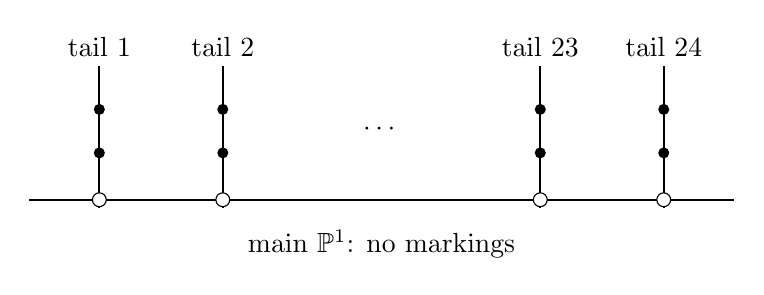
\begin{tikzpicture}[x=1.12cm,y=0.85cm]
 \draw[thick] (0,0) -- (8,0);
 \foreach \x/\lab in {0.8/1,2.2/2,5.8/23,7.2/24} {
  \draw[thick] (\x,-0.12) -- (\x,2);
  \draw[fill=white] (\x,0) circle (2.5pt);
  \fill (\x,0.7) circle (2pt);
  \fill (\x,1.35) circle (2pt);
  \node[above] at (\x,2) {tail $\lab$};
 }
 \node at (4,1.05) {$\cdots$};
 \node[below] at (4,-0.3) {main $\PP^1$: no markings};
\end{tikzpicture}
\caption{The distinguished fiber $D_*$ on $Y$, after the base change of index two and
one blowup at each collision. Each of the $24$ rational tails has two
markings (solid dots) and one node on the main component (open circles).
The middle $20$ tails are omitted. The cover constructed in \Cref{sec:surface}
is unramified at the nodes and can branch only at the markings. Its
inverse image may have a different incidence graph.}
\label{fig:distinguished-fiber}
\end{figure}


\begin{lemma}\label{lem:distinguished-meridians}
Every meridian around a component of $D_*$ has trivial image under $\rho_0$.
\end{lemma}

\begin{proof}
A main-component meridian is represented by the circuit along the fixed exterior section, so it is killed by \eqref{eq:rho-zero}.

For a tail use the blowup chart $w=uv$. A meridian at a sufficiently large fixed slope $v=c$ is represented downstairs by
\[
 u=\varepsilon e^{i\theta},\qquad
 w=c\varepsilon e^{i\theta},\qquad 0\le\theta\le2\pi.
\]
Choose $|c|$ larger than the two branch slopes and then choose $\varepsilon$ small. Trivialize the pair motion by an isotopy supported inside the circle containing the two marks but not this meridian. In this trivialization the loop is the base circuit followed by one full pair-boundary loop, up to conjugacy and the choice of multiplication convention. The base circuit is killed by the section splitting; the pair boundary is killed by the pinching map. Both factors therefore have trivial image.
\end{proof}

\subsection{The remaining boundary relations}

There are finitely many components of $D$ outside $D_*$. Choose based meridians $\mu_1,\ldots,\mu_b$ for them, and choose lifts $\widetilde\mu_i\in L$ of $\rho_0(\mu_i)\in Q_0$. These lifts exist since $L\to Q_0$ is surjective. Choose an integer $e$ so large that
\begin{equation}\label{eq:boundary-cost}
 b\,t^{2^e}<\frac1{100},
\end{equation}
and impose the additional relators $\widetilde\mu_i^{2^e}$.
This is the high-power method underlying Golod's construction
\citep{Golod1964}, applied here to the finitely many boundary elements.
Each added relator has degree at least $2^e$ by
\eqref{eq:degree-rules}. Denote the resulting pro-2 quotient by $Q$.

\begin{proposition}\label{prop:infinite-quotient}
The group $Q$ is infinite. The homomorphism
\[
 \rho:\pi_1(U)\longrightarrow Q
\]
induced by $\rho_0$ has dense image on every punctured fiber. Each component meridian of $D$ has finite image, and every component meridian of $D_*$ has trivial image.
\end{proposition}

\begin{proof}
Only infinitude remains to prove. The generators of $L$ have polynomial $P(t)$ and the involution relators have cost at most $tG(t)$, where \Cref{prop:involution} gives
\[
 P(t)=(1+t)G(t),\qquad
 G(t)=3t(1+t)(1+t^2)^2.
\]
At the rational value \eqref{eq:t-choice}, $t^2>3/50$, so
\[
 G(t)>
 \frac{3\cdot49\cdot249\cdot53^2}{200^2\cdot50^2}
 =\frac{102817827}{100000000}
 >\frac{257}{250}.
\]
The complete weighted expression in \Cref{lem:weighted-gs} is therefore less than
\[
 1-P(t)+tG(t)+\frac1{100}+\frac1{100}
 =1-G(t)+\frac1{50}
 <-\frac1{125}<0.
\]
The infinite monodromy-relator family is finite in each bounded degree and has convergent cost by \eqref{eq:monodromy-cost}. The remaining families are finite. All hypotheses of \Cref{lem:weighted-gs} hold, proving that $Q$ is infinite. Passage to the quotient preserves all earlier equalities and the density of each fiber image.
\end{proof}

Notice that $e$ is chosen after the finite cover and compactification. Thus their possibly large number of boundary components introduces no circular parameter choice. The surface construction now uses only the finite local images and the infinite fiber image recorded in \Cref{prop:infinite-quotient}.

\section{The projective surface and its rational fiber}
\label{sec:surface}

We now turn the quotient of \Cref{prop:infinite-quotient} into a
fundamental-group image on a smooth projective surface.  The construction
must retain the distinguished fiber: its rational components will lift
compactly, while the fundamental group of their union will have infinite
image.

Recall the inputs.  The complement $U=Y\setminus D$ lies in a smooth
connected projective surface $Y$, the boundary $D$ has simple normal
crossings, and
\[
  \rho:\pi_1(U)\longrightarrow Q
\]
has dense image in an infinite pro-$2$ group.  Its restriction to a
punctured smooth fiber also has dense image.  Every component meridian of
$D$ has finite image, and the meridians of the distinguished fiber
$D_*$ have trivial image.  This fiber consists of an unmarked main
sphere and $24$ tails, each meeting the main sphere once and carrying
two horizontal markings.

\subsection{A finite cover that kills all compactification meridians}

At a crossing, two commuting meridians may have relations that neither
cyclic subgroup detects separately.  We therefore choose a finite
quotient that detects the entire local group at every boundary point.

\begin{lemma}[Finite local detection and descent]
\label{lem:local-detection}
Let $Y$ be a smooth connected projective complex surface, let $D$ be a
simple-normal-crossings divisor, and put $U=Y\setminus D$.  Suppose
$\rho:\pi_1(U)\to Q$ has dense image in a profinite group and sends
every component meridian of $D$ to an element of finite order.
There is a finite quotient $Q\twoheadrightarrow P_f$ with the following
properties.
\begin{enumerate}
  \item The quotient is injective on the image under $\rho$ of every
  sufficiently small local boundary-complement group.
  \item The connected finite cover
  $\pi:U'\to U$ defined by
  $\ker(\pi_1(U)\to P_f)$ extends to a projective morphism
  $p:X\to Y$, where $X$ is smooth and connected and
  $D_X=X\setminus U'$ is a simple-normal-crossings divisor.
  \item Writing $i:U'\hookrightarrow X$ for inclusion, there is a
  homomorphism $\rho_X:\pi_1(X)\to Q$ such that
  \begin{equation}
    \rho_X\circ i_* = \rho\circ\pi_*.
    \label{eq:rho-descent}
  \end{equation}
\end{enumerate}
Moreover, the resolution used to construct $X$ can be chosen to preserve
every open subset of the normalization on which the surface is smooth
and its reduced boundary has simple normal crossings.
\end{lemma}

\begin{proof}
We first find a finite quotient detecting all local boundary images,
then compactify and resolve the corresponding cover, and finally
check that the original quotient map kills every new boundary
meridian.

Choose a small coordinate polydisk $V$ about a point of $D$.  Its
boundary complement is
\[
  V\setminus D\simeq(\Delta^*)^r\times\Delta^{2-r},
  \qquad r\in\{1,2\}.
\]
After choosing an access path in $U$, let
$A_V\subset Q$ be the image of its fundamental group.  This group is
generated by $r$ commuting finite-order elements, so it is finite.
Only finitely many such images occur up to conjugacy: there is one
meridian type on the smooth part of each boundary component and one
local group at each crossing.  The smooth part of an irreducible
component, with its finitely many crossings removed, is connected;
moving the access path along it conjugates the local group.

For every nonidentity element in representatives of these finite
groups, choose an open normal subgroup of $Q$ that does not contain
it.  Their finite intersection $N$ is open and normal.  It satisfies
\begin{equation}
  N\cap gA_Vg^{-1}=\{1\}
  \qquad(g\in Q)
  \label{eq:local-detection}
\end{equation}
for every local group.  Set $P_f=Q/N$.  Density makes the map
$\pi_1(U)\to P_f$ surjective, so its kernel defines a connected
finite Galois cover $\pi:U'\to U$.

The cover has the complex structure obtained by lifting local charts.
It is algebraic and finite \emph{\'etale} by the Riemann existence
theorem for complex varieties
\citep[Expos\'e XII, Th\'eor\`eme 5.1]{SGA1}.  This theorem applies
to the nonproper surface $U$.  Normalize $Y$ in the function field of
$U'$ and denote the resulting morphism by $n:\overline Y\to Y$.
It is finite: complex varieties are Nagata, so finiteness of relative
normalization applies to the finite-type morphism $U'\to Y$
\citep[Tag 03GR]{StacksProject}.
Its restriction over $U$ is $U'$, because the latter is already normal.
Finite morphisms are projective, so $\overline Y$ is projective
\citep[Tag 0B3I]{StacksProject}.

Resolve $\overline Y$ by projective blowups, leaving its smooth locus
unchanged; strong resolution in characteristic zero has this
prescribed-open property \citep[pp.~822--823]{EncinasHauser2002}.
Next resolve the reduced boundary on the resulting smooth surface.
For curves on a smooth surface this can be done by point blowups:
resolve the singular component germs, decrease tangency intersection
multiplicities, and separate crossings of three or more branches
\citep[Tag 0BIC and its proof]{StacksProject}.
Choose these centers only where the boundary is not already simple
normal crossings.  Thus this additional operation preserves every
open subset on which the pair was already smooth with simple normal
crossings.  We obtain
\[
  X\xrightarrow{\ r\ }\overline Y
    \xrightarrow{\ n\ }Y,
  \qquad p=n\circ r,
\]
with $X$ smooth and projective and with $D_X$ a
simple-normal-crossings divisor.  The dense open set $U'$ is unchanged,
so $X$ is connected.

We prove the factorization, including the meridians of resolution
exceptional curves.  The inclusion $i$ is surjective on fundamental
groups: a loop can be perturbed off a real-codimension-two divisor.
Its kernel is normally generated by the component meridians of $D_X$.
Indeed, perturb a null-homotopy disk relative to its boundary so that
it avoids the finitely many crossings of $D_X$ and meets its smooth
part transversely.  Deleting small disks around the finitely many
intersection points expresses its boundary loop as a product of
conjugates of meridians and their inverses.

Let $E$ be any component of $D_X$, choose a smooth point $x\in E$
away from the other components, and take a small transverse disk
$T$ through $x$ with $T\setminus\{x\}\subset U'$.  Choose a boundary
polydisk $V$ about $p(x)$ downstairs.  By shrinking $T$, we may assume
$p(T)\subset V$.  Consequently the projection of a small meridian
in $T\setminus\{x\}$ lies in $V\setminus D$.  After including its
access path, its $Q$-image belongs to a conjugate of $A_V$.
This argument applies also when $E$ is exceptional and is contracted
to a boundary point.

The projected meridian has trivial image in $P_f$, since its lift is
a closed loop in $U'$.  Its $Q$-image therefore lies in both $N$ and
a conjugate of $A_V$, and is trivial by
\eqref{eq:local-detection}.  All generators of $\ker i_*$ are thus
killed by $\rho\circ\pi_*$.  This proves
\eqref{eq:rho-descent}.
\end{proof}

Apply \Cref{lem:local-detection} to the map supplied by
\Cref{prop:infinite-quotient}.  Retain its notation
$P_f,N,U',\overline Y,X,p,\rho_X$.  We next verify that the
normalization is already smooth along the distinguished fiber, so
that the resolution can preserve it.

\subsection{The distinguished fiber remains a union of spheres}

\begin{lemma}
\label{lem:rational-special-fiber}
Let $h:X\to C'$ be the composite of $p$ and $Y\to C'$.  The
resolution can be chosen so that the reduced fiber
\[
  Z=h^{-1}(c_*)_{\mathrm{red}}
\]
has only smooth rational irreducible components and ordinary
transverse crossings.
\end{lemma}

\begin{proof}
Every vertical meridian along $D_*$ is trivial in $Q$, and hence in
$P_f$, by \Cref{lem:distinguished-meridians}.  We describe the
normalization locally at every kind of point of $D_*$.  The
restriction of the Galois cover to a boundary-complement polydisk
is classified by its local meridian homomorphism to $P_f$; its
connected components correspond to cosets of the local image.

At a smooth unmarked point of $D_*$, the sole meridian is trivial.
Every connected local cover therefore extends as a copy of the
polydisk.  At a node between the main component and a tail, both
vertical meridians are trivial, and the same assertion holds.

At a horizontal--vertical intersection choose coordinates $(u,v)$
with the vertical curve $u=0$ and the horizontal marking $v=0$.
The $u$-meridian is trivial.  If the image of the $v$-meridian has
order $e$, the kernel of the local map $\Z^2\to P_f$ is
$\Z\times e\Z$.  Each connected local cover thus has the finite
normal extension
\begin{equation}
  (u,w)\longmapsto (u,v)=(u,w^e).
  \label{eq:distinguished-local-cover}
\end{equation}
This extension is smooth, and its reduced boundary is $uw=0$.
Analytification preserves finiteness and normality
\citep[Expos\'e XII, Propositions~2.1(vi) and 3.2(vi)]{SGA1}.
Thus the local extensions just described agree with $\overline Y$ by
uniqueness of finite normal extension
\citep[Expos\'e XII, Proposition~5.3]{SGA1}. The entire preimage of $D_*$
lies in the smooth simple-normal-crossings locus of the normalized
pair.  The resolution in \Cref{lem:local-detection} can be the
identity on this open neighborhood.



Consider now an irreducible component above the main sphere.
Its map to that sphere is unramified, including at the attaching
nodes, and there are no horizontal markings on the main component.
It is therefore a connected unramified cover of $\PP^1$, hence a
sphere mapping with degree one.  A component above a tail can branch
only at its two horizontal markings, and is unramified at the
attaching node.  Removing those two points downstairs and all their preimages upstairs
gives a connected finite cover of $\C^*$. Its covering subgroup is
$d\Z\subset\Z$.  Thus it is the covering $z\mapsto z^d$ of $\C^*$,
whose smooth compactification is $\PP^1$.

There are no additional components from resolution over $D_*$.
The local models show that the components just identified are
smooth and meet only in ordinary transverse crossings.  This
proves the assertion about $Z$.
\end{proof}

\subsection{Infinite image on the compact fiber}

Although $D_*$ is a tree of spheres, a degree-$d$ component above
one of its tails meets $d$ distinct degree-one lifts of the main
sphere: the attaching node has $d$ distinct preimages. The incidence
graph upstairs therefore need not be a tree. For a connected nodal
union of simply connected components, van Kampen identifies its
fundamental group with that of its dual graph, which has one vertex
for each component and one edge for each node. We now prove that
some connected component of $Z$ has infinite fundamental-group image
in $X$.

\begin{lemma}
\label{lem:infinite-special-image}
Let $Z=h^{-1}(c_*)_{\mathrm{red}}$ be the rational nodal fiber of
\Cref{lem:rational-special-fiber}. Some connected component $Z_0$ of $Z$ satisfies
\[
  \bigl|\im\bigl(\pi_1(Z_0)\longrightarrow\pi_1(X)\bigr)\bigr|
  =\infty.
\]
\end{lemma}

\begin{proof}
Let $F_s\subset U$ be a punctured smooth fiber, with $s\in B'$,
and choose access paths when comparing its group with $\pi_1(U)$.
Its image under $\rho$ is dense in $Q$ by
\Cref{prop:infinite-quotient}.  In particular its image in $P_f$
is all of $P_f$, so its inverse image $F'_s\subset U'$ is
connected.  Under the covering inclusion, its group is the
preimage of $N$ in $\pi_1(F_s)$.  Thus the image of
$\pi_1(F'_s)$ in $Q$ is
\[
  \rho\bigl(\pi_1(F_s)\bigr)\cap N.
\]
It is dense in $N$, because $N$ is open and the fiber image is
dense in $Q$.  The group $N$ is infinite: a finite open subgroup
would make its finite-index overgroup $Q$ finite.  Consequently
the image of $\pi_1(F'_s)$ in $Q$ is infinite.  By
\eqref{eq:rho-descent}, its image in $\pi_1(X)$ is infinite as
well.

We transfer this conclusion to $Z$ using an explicit
deformation-retract neighborhood.  Regard $X$ as a compact real analytic
manifold and $Z$ as a closed semianalytic subset.  This pair admits a
compatible finite triangulation
\citep[Section 3, Theorem 2, p.~464]{Lojasiewicz1964}.
Write it as a finite simplicial pair $(\mathcal K,\mathcal A)$,
and barycentrically subdivide so that $\mathcal A$ is a full
subcomplex: any simplex whose vertices belong to $\mathcal A$
belongs to $\mathcal A$.  For a point of $|\mathcal K|$, let $s_{\mathcal A}$
be the sum of its barycentric coordinates at vertices of
$\mathcal A$.  On the open neighborhood
\[
  V=\{s_{\mathcal A}>0\}
\]
retain those coordinates, divide them by $s_{\mathcal A}$, and
set all other coordinates to zero.  Fullness ensures that the
result belongs to $|\mathcal A|$.  The straight-line homotopy
inside each simplex gives a strong deformation retraction
$V\to Z$.  In particular the inclusion of $V$ into $X$ is
homotopic to a map through $Z$.

Properness of $h$ supplies the needed containment of nearby
fibers.  The set $h(X\setminus V)$ is closed in $C'$ and does
not contain $c_*$.  Hence every whole fiber over a sufficiently
small neighborhood of $c_*$ lies in $V$.  Choose $s\in B'$ in
this neighborhood.  Its connected punctured lifted fiber
$F'_s$ lies in one connected component of $V$; the deformation
retraction takes that component into a connected component
$Z_0$ of $Z$.  Therefore its inclusion-induced homomorphism to
$\pi_1(X)$ factors, up to a change-of-basepoint conjugation,
through $\pi_1(Z_0)$.  Since the former has infinite image, so
does the latter.
\end{proof}

\begin{proof}[Proof of \Cref{thm:main}]
The construction above gives a smooth connected projective surface
$X$.  By \Cref{lem:rational-special-fiber,lem:infinite-special-image},
it contains a connected nodal curve $Z_0$ with smooth rational
irreducible components and infinite image in $\pi_1(X)$.

\Cref{lem:rational-hull} now applies to $(X,Z_0)$.  In the simply
connected universal cover $\widetilde X$, every connected component
$W$ above $Z_0$ is a closed noncompact locally finite union of
compact rational curves.  For every $w\in W$, the holomorphic
hull of $\{w\}$ contains $W$ and is noncompact.  This proves all
the assertions of \Cref{thm:main}.
\end{proof}

\bibliographystyle{plainnat}
\bibliography{references}
\end{document}
